\documentclass[11pt,a4paper]{article}
\usepackage[utf8]{inputenc}
\usepackage[T1]{fontenc}
\usepackage[spanish,es-noshorthands]{babel}
\usepackage{amsmath,amssymb,amsthm}
\usepackage{bm}
\usepackage{geometry}
\geometry{margin=2.5cm}
\usepackage{graphicx}
\graphicspath{{../figuras/}}
\usepackage{float}
\usepackage{xcolor}
\usepackage{hyperref}
\hypersetup{colorlinks=true,linkcolor=blue!50!black,citecolor=blue!50!black,urlcolor=blue!50!black}
\usepackage{enumitem}
\usepackage{booktabs}
\newtheorem{definition}{Definición}
\newtheorem{remark}{Observación}
\newcommand{\R}{\mathbb{R}}
\newcommand{\thetavec}{\bm{\theta}}
\newcommand{\transp}{^{\top}}
\newcommand{\promptIA}[1]{\begin{center}\fcolorbox{gray}{gray!8}{\parbox{0.9\linewidth}{\small\textbf{[FIGURA -- PROMPT IA]}\\[2pt]#1}}\end{center}}
\title{\textbf{B5 --- Neuroestimulación y control en lazo cerrado}\\[2pt]\large Del estímulo óptico al gemelo digital: por qué identificar antes de controlar}
\author{Proyecto Wilson--Cowan --- Iniciación a la I+D ITBA}
\date{\today}
\begin{document}
\maketitle
\tableofcontents
\bigskip

\noindent\textbf{Requisitos previos:} B3 (modelo de Wilson--Cowan), B4 (régimen theta--gamma). \textbf{Conecta con:} M5 (Neural ODE como planta identificada), P4 (implementación \texttt{neural\_ode}).

\bigskip
\noindent Este documento es el \emph{para qué} del proyecto. Todo lo anterior --- escribir las ecuaciones de WC, integrarlas numéricamente, identificar sus 10 parámetros, diagnosticar cuáles se recuperan y cuáles no --- existe para habilitar un objetivo concreto: \textbf{fabricar estímulos que empujen a una población neuronal hacia un ritmo deseado, en tiempo real, corrigiendo sobre la marcha}. Eso es neuroestimulación en lazo cerrado. Acá conectamos la biología del estímulo (optogenética, DBS) con la ingeniería de control, y mostramos el resultado central del proyecto: la fragilidad para identificar $w_{II}$ \emph{no} se propaga al control.

\section{Optogenética: control óptico de neuronas}

\begin{definition}[Optogenética]
Técnica que hace a neuronas específicas sensibles a la luz insertándoles genéticamente una \emph{opsina} (una proteína-canal fotosensible, p.\ ej.\ la channelrhodopsina-2, ChR2). Al iluminar el tejido con luz de la longitud de onda adecuada, esos canales se abren y la neurona se despolariza (o se hiperpolariza, según la opsina) \emph{con precisión de milisegundos} \cite{boyden2005,deisseroth2011}.
\end{definition}

\paragraph{Intuición.} La opsina es un interruptor molecular accionado por fotones. La luz llega por una fibra óptica implantada; mientras el LED o láser está encendido, la corriente entra; cuando se apaga, se corta. A diferencia de una droga (que difunde lento y afecta a todo lo que encuentre), la optogenética es \emph{rápida} y \emph{selectiva}: solo responden las neuronas que expresan la opsina, y solo mientras hay luz.

\paragraph{Por qué esto le pone un corsé a las señales realizables.} Acá está el punto que conecta la biología con toda la librería de estímulos del proyecto. El actuador optogenético tiene dos limitaciones físicas duras:
\begin{itemize}[leftmargin=1.4em]
  \item \textbf{On/off (conmutado).} El LED enciende o apaga. La modulación fina y continua de intensidad es difícil y ruidosa; en la práctica el estímulo se piensa como una señal \emph{conmutada} entre niveles.
  \item \textbf{No negativo ($\geq 0$).} La luz aporta activación; no se puede ``iluminar en negativo''. El estímulo $u(t)$ es una cantidad de fotones, y eso es siempre $\geq 0$. (Inhibir requiere \emph{otra} opsina, no un valor negativo de la misma.)
\end{itemize}

En las ecuaciones de WC (ver B3) los estímulos $P(t)\to E$ y $Q(t)\to I$ representan justamente esa entrada externa. Si el proyecto quiere que sus resultados sean \emph{traducibles al banco óptico}, los estímulos de identificación tienen que respetar esas dos restricciones. Por eso la librería del proyecto está hecha de señales \textbf{conmutadas y no negativas}:
\begin{itemize}[leftmargin=1.4em]
  \item \textbf{pulsos} (escalones on/off);
  \item \textbf{PRBS} (\emph{Pseudo-Random Binary Sequence}): secuencia binaria pseudoaleatoria --- salta entre dos niveles $\geq 0$;
  \item \textbf{APRBS} (\emph{Amplitude-modulated PRBS}): PRBS con varios niveles de amplitud, todos $\geq 0$, para excitar también la no linealidad de la sigmoidea;
  \item \textbf{theta--gamma}: ráfagas gamma moduladas por una envolvente theta, todas positivas (ver B4).
\end{itemize}

\begin{remark}[El chirp suave NO es realizable con optogenética]
Un \emph{chirp} (sinusoide de frecuencia creciente) es la señal ideal para identificación en teoría de sistemas: barre frecuencias suavemente y excita todos los modos. Pero es una señal \emph{continua y con parte negativa}. Con un LED on/off que solo aporta luz $\geq 0$ no se puede reproducir un chirp suave. Por eso en el proyecto el chirp aparece \emph{únicamente como trayectoria de test} (validación limpia, ver \texttt{fit\_chirp\_test.png} en los materiales de identificación), nunca como estímulo de excitación destinado al banco real. La restricción biológica del actuador \textbf{define qué entradas tiene sentido diseñar}.
\end{remark}

\promptIA{Esquema didáctico de optogenética. En el centro, una neurona piramidal (soma triangular, dendritas arriba, axón abajo) con su membrana punteada de pequeños canales-proteína incrustados (las opsinas / channelrhodopsina), representados como cilindros azules que atraviesan la bicapa lipídica. Desde arriba baja una \textbf{fibra óptica} (cilindro gris delgado con un núcleo claro) que termina justo sobre la neurona y emite un cono de \textbf{luz azul} ($\sim$470 nm) que ilumina la zona de los canales. Flechas pequeñas de iones (Na$^+$, Ca$^{2+}$) entrando por los canales abiertos bajo la luz. Abajo, una mini-línea de tiempo con un tren de pulsos cuadrados on/off etiquetado ``estímulo óptico ($\geq 0$, conmutado)'', y al lado un registro de disparos de la neurona alineado a los pulsos. Estilo: ilustración científica limpia, fondo blanco, etiquetas en español (``opsina (ChR2)'', ``fibra óptica'', ``luz azul 470 nm'', ``membrana''). Paleta sobria azul/gris.}

\section{DBS: estimulación cerebral profunda}

\begin{definition}[Deep Brain Stimulation, DBS]
Terapia que consiste en implantar quirúrgicamente un electrodo en un núcleo cerebral profundo y aplicar pulsos \emph{eléctricos} de alta frecuencia (típicamente $\sim$130--180 Hz) mediante un generador implantado. Es un tratamiento clínico establecido, sobre todo para los síntomas motores de la \textbf{enfermedad de Parkinson} \cite{kuncel2004}.
\end{definition}

\paragraph{Cómo se diferencia de la optogenética.} La DBS es \emph{eléctrica} (no óptica) y \emph{no selectiva}: el campo eléctrico afecta a todo el tejido alrededor del electrodo, sin distinguir tipos celulares. La optogenética, en cambio, es óptica y genéticamente dirigida --- solo actúa sobre las neuronas que expresan la opsina. La contrapartida: la DBS \emph{ya se usa en humanos} desde hace décadas, mientras que la optogenética es, por ahora, sobre todo una herramienta de investigación (requiere modificación genética).

\paragraph{El problema de elegir los parámetros.} En DBS clínica hay que fijar amplitud, ancho de pulso y frecuencia del estímulo. Estos parámetros se ajustan hoy en gran medida por prueba y error, buscando el equilibrio entre eficacia terapéutica y efectos secundarios \cite{kuncel2004}. Esta dificultad --- ``¿qué estímulo aplico?'' --- es exactamente la pregunta que el enfoque \emph{basado en modelo} de este proyecto intenta responder de forma principiada: si tengo un modelo de la planta, puedo \emph{calcular} el estímulo en vez de tantear.

\section{Lazo abierto vs.\ lazo cerrado}

Toda neuroestimulación cae en una de dos categorías, según si mira o no lo que está pasando en el cerebro.

\paragraph{Lazo abierto (\emph{open-loop}).} Se aplica un estímulo prefijado --- por ejemplo, el tren de pulsos de 130 Hz de la DBS clásica --- \emph{sin importar el estado momentáneo} del sistema. Es simple y robusto, pero ciego: estimula igual esté el paciente en reposo o en plena crisis, y por eso gasta energía de más y puede producir efectos secundarios evitables.

\paragraph{Lazo cerrado (\emph{closed-loop} / adaptativo).} Se cierra el ciclo
$$\text{\textbf{medir}} \;\longrightarrow\; \text{\textbf{decidir}} \;\longrightarrow\; \text{\textbf{estimular}} \;\longrightarrow\; (\text{el cerebro cambia})\;\longrightarrow\; \text{medir}\dots$$
Se registra continuamente una señal del cerebro (p.\ ej.\ la actividad de la población), un controlador \emph{decide} qué estímulo aplicar según ese estado, y actúa. Luego vuelve a medir. Las ventajas son directas:
\begin{itemize}[leftmargin=1.4em]
  \item \textbf{Adaptativo:} responde al estado real, no a un guion fijo. Estimula fuerte cuando hace falta y afloja cuando no.
  \item \textbf{Menos energía y menos efectos secundarios:} al estimular solo lo necesario, se reduce la dosis total.
  \item \textbf{Bajo demanda:} el ejemplo canónico es el control optogenético \emph{on-demand} de convulsiones espontáneas: el sistema detecta el inicio de una crisis y dispara el estímulo justo para abortarla \cite{krookmagnuson2013}.
\end{itemize}

En este proyecto, la referencia a seguir es un \textbf{ritmo theta--gamma} (ver B4), y el ``medir'' son las tasas $I(t)$ y $E(t)$ de las poblaciones. El controlador que cierra el lazo es un IMC, que describimos abajo.

\promptIA{Diagrama de bloques de neuroestimulación en lazo cerrado, estilo diagrama de control clásico, horizontal, izquierda a derecha. Bloque ``Referencia $r(t)$: ritmo theta--gamma deseado'' entra a un nodo suma circular ($\Sigma$) con signo $+$; del nodo sale la señal de error hacia un bloque rectangular ``Controlador IMC''. Del controlador sale ``estímulo $P(t), Q(t)$ (óptico, $\geq 0$)'' hacia un bloque ``Cerebro / población neuronal (planta)'' dibujado como una cabeza estilizada con una fibra óptica implantada. De la planta sale ``$y(t)=E(t)-I(t)$ (actividad medida)'', que se realimenta hacia atrás por una línea inferior etiquetada ``sensor / registro'' de vuelta al nodo suma con signo $-$. Marcar bien las tres etapas con etiquetas grandes debajo del lazo: \textbf{MEDIR} (bajo el sensor), \textbf{DECIDIR} (bajo el controlador), \textbf{ESTIMULAR} (bajo la flecha de estímulo). Estilo: líneas limpias, cajas rectangulares, fondo blanco, etiquetas en español. Paleta azul/gris sobria.}

\section{Por qué identificar antes de controlar}

Acá se junta todo el proyecto. La cadena lógica es: \emph{para controlar bien, primero necesito un modelo de la planta que estoy controlando}.

\paragraph{El modelo identificado es un ``gemelo digital''.} El Neural ODE que identificamos (ver M5, P4) es una réplica \emph{in silico} de la dinámica neuronal real: mismos estados $I, E$, misma estructura de WC, con los 10 parámetros $\thetavec$ estimados de los datos. Ese gemelo digital cumple dos roles:
\begin{enumerate}[leftmargin=1.6em]
  \item Es la \textbf{planta} sobre la que se \emph{diseña} y se \emph{prueba} el controlador antes de tocar tejido real (barato, seguro, reproducible).
  \item Aporta los \textbf{pesos $\thetavec$} que el controlador usa internamente para saber cómo responde el sistema al estímulo.
\end{enumerate}
Sin modelo, uno estaría de vuelta en el ``prueba y error'' de la DBS clásica. Con modelo, se puede \emph{calcular} el estímulo.

\subsection*{El controlador IMC del proyecto, a grandes rasgos}

El controlador es un \textbf{IMC} (\emph{Internal Model Control}) con \emph{linealización por realimentación}, portado del código MATLAB del tutor. Tiene dos capas con roles muy distintos --- y esa separación es la clave de todo lo que sigue.

\paragraph{(a) Cancelación del acoplamiento (feedforward) --- \emph{usa} $\thetavec$.} WC tiene, dentro de la sigmoidea, un término de acoplamiento entre poblaciones: $w_{IE}E - w_{II}I$ para la población $I$, y $w_{EE}E - w_{EI}I$ para la $E$. La idea del IMC es \textbf{restar ese término con el propio estímulo}, usando los pesos identificados:
$$Q = u_q - (w_{IE}\,E - w_{II}\,I), \qquad P = u_p - (w_{EE}\,E - w_{EI}\,I).$$
Si la cancelación fuera perfecta, la dinámica en lazo cerrado quedaría \emph{lineal y desacoplada}, y el resto del control sería trivial. Esta capa es la que \emph{necesita} los parámetros $\thetavec$ (los pesos y la sigmoidea; notablemente \emph{no} usa las constantes de tiempo $\tau_e, \tau_i$).

\paragraph{(b) Realimentación PI con acción integral --- \emph{no usa} $\thetavec$.} Sobre lo anterior actúa un lazo proporcional-integral clásico. Con integradores $Z_1, Z_2$ que acumulan el error de seguimiento:
$$\dot Z_1 = r_I - I, \qquad \dot Z_2 = r_E - E,$$
$$U^{lti}_I = k_{pI}(r_I - I) + k_{iI}Z_1, \qquad U^{lti}_E = k_{pE}(r_E - E) + k_{iE}Z_2.$$
Esta capa \textbf{no depende de $\thetavec$ en absoluto}: es puro error medido $r - y$ y su integral en el tiempo. El estado aumentado $[Z_1, Z_2, I, E]$ se integra con RK4.

La observación crucial --- que desarrollamos en la próxima sección --- es que estas dos capas reparten el trabajo de forma muy conveniente: el feedforward (que sí necesita $\thetavec$) solo mejora el \emph{transitorio}, mientras que la acción integral (que \emph{no} necesita $\thetavec$) garantiza el \emph{régimen permanente}.

\section{El resultado clave: la fragilidad de \texorpdfstring{$w_{II}$}{wII} no se propaga al control}

\paragraph{El objetivo del proyecto.} Inducir y mantener un \textbf{ritmo theta--gamma} en la población de WC mediante estímulos realizables, cerrando el lazo con el gemelo digital identificado. Ese es el entregable de la validación orientada al control (objetivo OE3).

\paragraph{El cuello de botella, recordado.} La identificación tiene un punto débil bien caracterizado (ver M6): el peso de autoinhibición $w_{II}$ es \emph{casi irrecuperable} de los datos. El diagnóstico Fisher+SVD lo predice (valle plano de la FIM) y el ruido lo confirma: a $\sigma=0.10$ el error de $w_{II}$ en la estimación ingenua llega a \textbf{superar el 100\,\%}. Leído como problema de identificación, esto es una mala noticia.

\paragraph{El giro.} Pero el objetivo final \emph{no} es identificar $w_{II}$: es \emph{controlar}. Y para controlar, la acción integral no necesita conocer $\thetavec$. Retomando el argumento de la sección anterior: si el controlador se construye con $\hat{\thetavec} \neq \thetavec$, la cancelación feedforward es imperfecta y deja un residuo
$$\Delta Q = (\hat w_{IE}-w_{IE})\,E - (\hat w_{II}-w_{II})\,I$$
(análogo para $\Delta P$). Ese residuo entra al lazo como una \textbf{perturbación de carga} aditiva. Y por el \emph{principio del modelo interno}, un integrador en el lazo lleva el error de seguimiento a cero ante perturbaciones y referencias tipo escalón, \textbf{sin importar el valor exacto de los pesos}, siempre que el lazo siga estable. En una frase: \emph{el error de $\hat{\thetavec}$ se convierte en una perturbación acotada que el integrador absorbe; $\hat{\thetavec}$ solo afecta la calidad del feedforward (el transitorio), no la capacidad de seguir la referencia (el régimen permanente).}

\paragraph{La evidencia.} La matriz $2\times 2$ de configuraciones \{simulador, Neural ODE\} $\times$ \{$\hat{\thetavec}$ estimados, $\thetavec$ reales\} da un RMSE de seguimiento \textbf{casi idéntico} en toda referencia. El RMSE varía con la \emph{dificultad de la referencia} ($\sim$2--4$\times 10^{-2}$), no con la configuración. Aún más contundente: bajo ruido, mientras el error de $\hat w_{II}$ ingenuo escala hasta el 106\,\%, el RMSE de control se mantiene pegado al ideal ($\sim 3.3\times 10^{-2}$) en todos los niveles de ruido.

\begin{table}[H]
\centering
\small
\begin{tabular}{cccc}
\toprule
$\sigma$ (ruido) & error $\hat w_{II}$ ingenuo & error $\hat w_{II}$ mejorado & RMSE control ($I$ / $E$) \\
\midrule
0.00 & 0.4\,\%   & 0.1\,\% & $3.35 / 3.13 \times 10^{-2}$ \\
0.01 & 2.1\,\%   & 0.6\,\% & $3.35 / 3.14 \times 10^{-2}$ \\
0.05 & 19.3\,\%  & 1.2\,\% & $3.37 / 3.13 \times 10^{-2}$ \\
0.10 & 106.1\,\% & 8.9\,\% & $3.42 / 3.06 \times 10^{-2}$ \\
\bottomrule
\end{tabular}
\caption{La identificación de $w_{II}$ se degrada brutalmente con el ruido (columna 2), pero el seguimiento en lazo cerrado se mantiene en el nivel ideal (columna 4). La fragilidad de la identificación no se propaga al control.}
\label{tab:ruido}
\end{table}

\begin{figure}[H]
\centering
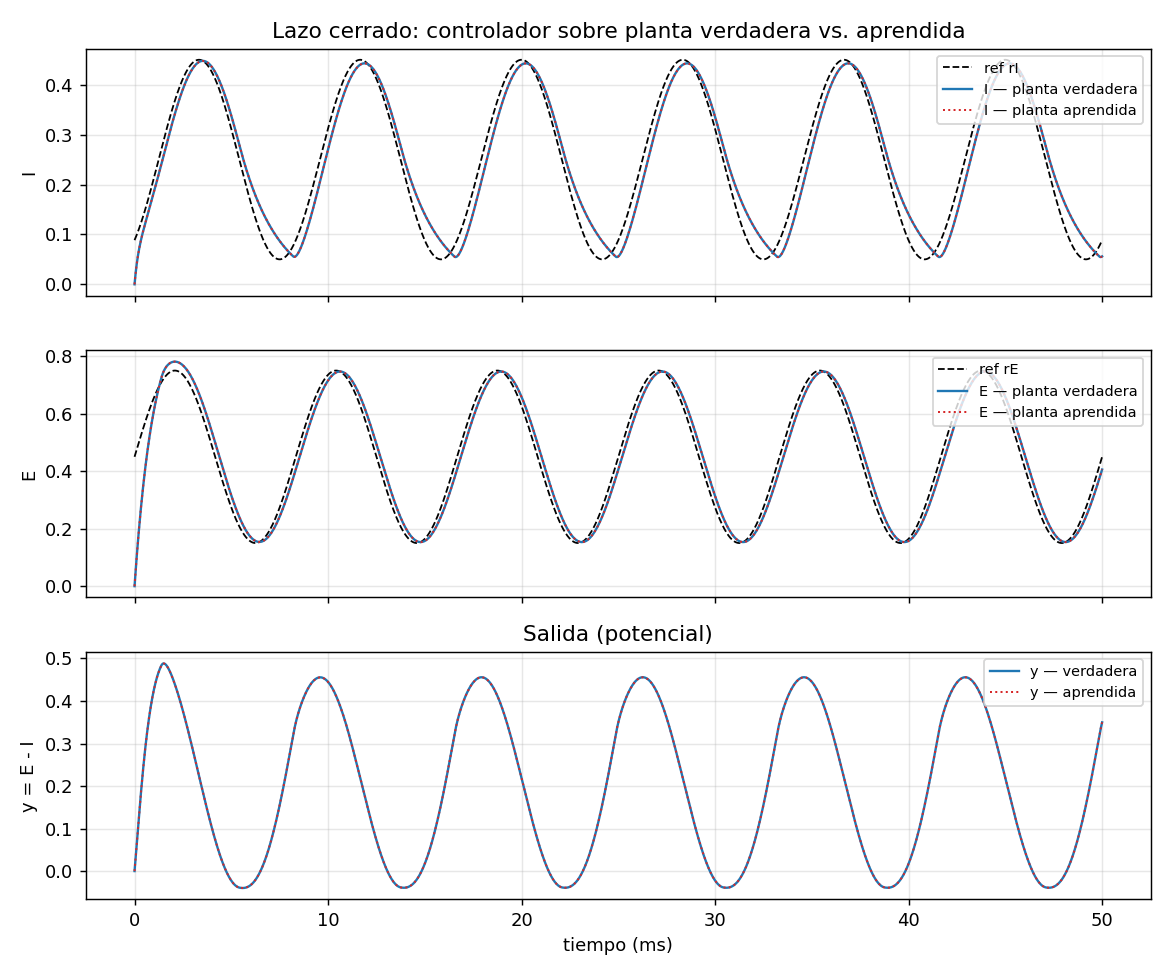
\includegraphics[width=0.75\linewidth]{closed_loop_compare.png}
\caption{Seguimiento en lazo cerrado con parámetros estimados $\hat{\thetavec}$ frente a los reales $\thetavec$: las trayectorias son prácticamente indistinguibles. La acción integral absorbe el error de estimación. (figura del proyecto)}
\label{fig:closedloop}
\end{figure}

\paragraph{Por qué esto da vuelta la lectura pesimista.} El cuello de botella de $w_{II}$ (ver M6) parecía un límite fatal del proyecto. Este resultado lo reencuadra: \textbf{$w_{II}$ es casi irrecuperable para identificar, pero para el objetivo real --- controlar --- no hace falta recuperarlo bien.} La debilidad de la identificación queda ``escondida'' detrás de la robustez del control.

\begin{remark}[La salvedad honesta]
La robustez es \emph{condicional a la estabilidad}, no infinita. Si $\hat{\thetavec}$ estuviera tan errado que la cancelación imperfecta desestabilizara el lazo (polos a la derecha), la acción integral ya no salvaría nada. Además, el esquema asume realimentación de estado completo ($I, E$ medidos directo); con ruido de medición fuerte haría falta un observador o EKF como capa extra. Y el análisis es para error de estimación \emph{estático}: el modelo es tiempo-invariante (confirmado por el tutor), así que la deriva paramétrica queda fuera de alcance.
\end{remark}

\section{Encuadre de novedad y antecedente cercano}

\paragraph{Qué aporta este proyecto.} La combinación específica es la contribución: identificar un modelo \emph{gray-box} de WC con Neural ODE, diagnosticar su identificabilidad con Fisher+SVD, y \emph{cerrar el lazo} mostrando que el cuello de botella de identificación no compromete el control. Es la cadena completa \textbf{identificar $\to$ diagnosticar $\to$ diseñar estímulo $\to$ controlar}, con estímulos pensados para ser realizables con optogenética.

\paragraph{El antecedente más cercano.} El \emph{Adaptive Stimulus Design} diseña estímulos óptimos para excitar una red neuronal recurrente (RNN) y así identificarla mejor --- es decir, aborda la parte de \emph{diseño de estímulo / OED} del problema. Pero se detiene ahí: es \emph{otro modelo} (una RNN genérica, no la estructura biofísica de WC) y \textbf{no incluye la etapa de control}. La novedad de este proyecto es precisamente unir la identificación diagnosticada con el control en lazo cerrado sobre un modelo neuronal interpretable, y usar esa unión para responder una pregunta que la sola identificación no puede: \emph{¿importa para el control que un parámetro sea no identificable?} La respuesta, aquí, es que no.

\begin{thebibliography}{9}

\bibitem{boyden2005} E.~S. Boyden, F.~Zhang, E.~Bamberg, G.~Nagel y K.~Deisseroth, ``Millisecond-timescale, genetically targeted optical control of neural activity'', \emph{Nature Neuroscience} 8:1263--1268, 2005.

\bibitem{deisseroth2011} K.~Deisseroth, ``Optogenetics'', \emph{Nature Methods} 8:26--29, 2011.

\bibitem{krookmagnuson2013} E.~Krook-Magnuson, C.~Armstrong, M.~Oijala e I.~Soltesz, ``On-demand optogenetic control of spontaneous seizures in temporal lobe epilepsy'', \emph{Nature Communications} 4:1376, 2013.

\bibitem{kuncel2004} A.~M. Kuncel y W.~M. Grill, ``Selection of stimulus parameters for deep brain stimulation'', \emph{Clinical Neurophysiology} 115(11):2431--2441, 2004.

\end{thebibliography}

\end{document}
